% compiler avec lualatex
\documentclass{matapli}
%\usepackage{marvosym}
%\usepackage[cam,a4,center]{crop}

\renewcommand{\numero}{123} %%% modifier   chaque numro
\renewcommand{\mois}{Novembre 2020}%%% modifier   chaque numro


\newcommand{\roundpic}[4][]{
  \tikz\node [circle, inner sep = 5pt, fill=white, draw=black, minimum width = #2,
  path picture = {
    \node [#1] at (path picture bounding box.center) {
      \includegraphics[width=#3]{#4}};
  }] {};
}
\pagestyle{empty}
\parindent0pt

\begin{document}

\newcommand\logo{
\includegraphics[width=0.4\paperwidth]{Logo.pdf}}
\newcommand\fond{
\includegraphics[width=1.1\paperwidth]{fond.pdf}}
\newcommand\numDate{\No \numero~~  --- ~~ \mois}
\begingroup
\fontspec{libertinussans}%[

\begin{tikzpicture}[overlay, remember picture]
  \node at (current page.center) {\fond};
  \node[anchor=north west,font=\Huge\bfseries,scale=3] at ($(current page.north west)+(4.7,-3.5)$) {MATAPLI};
  \node[anchor=north west] at ($(current page.north west)+(0.2,-0.2)$) {\logo};
  \node [circle, inner sep = 5pt, fill=white, draw=black, minimum width = 5cm,
   path picture = {
     \node [] at (path picture bounding box.center) {
       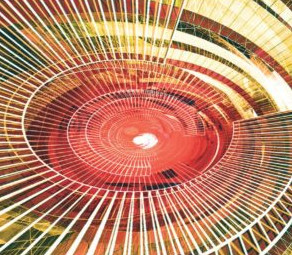
\includegraphics[width=5.5cm]{couverture.jpg}
     };
   }] at  ($(current page.south)+(-3,0.22\paperheight)$) {};
  \node [circle, inner sep = 5pt, fill=white, draw=black, minimum width = 9cm,
   path picture = {
     \node [] at (path picture bounding box.center) {
       
\includegraphics[width=9.4cm]{CIMPA.png}
   };
 }] at  ($(current page.south)+(1,0.5\paperheight)$) {};
   \node [circle, inner sep = 5pt, fill=white, draw=black, minimum width = 3cm,
   path picture = {
     \node [] at (path picture bounding box.center) {
       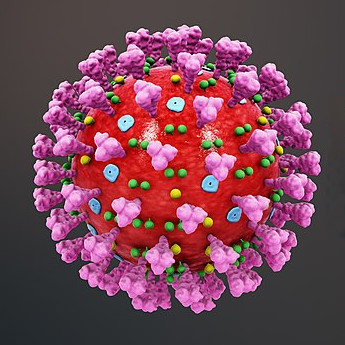
\includegraphics[width=3cm]{corona.jpg}};
   }] at  ($(current page.south)+(1.5,0.23\paperheight)$) {};
  \node[anchor=south east,color=black, font=\bfseries\Huge] at ($(current
  page.south east)-(0.5,-0.5)$) {\numDate};
\end{tikzpicture}
\endgroup



\newpage
\vspace*{-2cm}


\section*{Comité de rédaction}


\redacteurMatapli{Rédacteur en chef}{Julien \bsc{Salomon}}{Équipe ANGE, INRIA Paris}{\url{salomon@inria.fr}}

\redacteurMatapli{Rédacteur en chef adjoint}{Maxime \bsc{Chupin}}{CEREMADE, CNRS,  Université Paris-Dauphine}{\url{chupin@ceremade.dauphine.fr}}


\subsection*{Rédacteurs}


\redacteurMatapli{Congrès et colloques}{Thomas \bsc{Haberkorn}}{Fédération Denis Poisson, Université d'Orléans}{\url{thomas.haberkorn@univ-orleans.fr}}

\redacteurMatapli{Du côté de l'INRIA}{Arthur \bsc{Vidard}}{INRIA Paris}{\url{Arthur.Vidard@inria.fr}}

\redacteurMatapli{Du côté des écoles d'ingénieurs}{Emmanuel \bsc{Audusse} et Olivier \bsc{Laffite}}{LAGA, Université Paris XIII}{\url{eaudusse@yahoo.fr}, \url{lafitte@math.univ-paris13.fr}}

\redacteurMatapli{Du côté du réseau MSO}{Véronique \bsc{Maume-Deschamps}}{AMIES, 
Université Lyon 1, Institut Camille Jordan}{\url{veronique.maume-deschamps@agence-maths-entreprises.fr}}

\redacteurMatapli{Du côté des industriels}{Christian \bsc{Gout}}{INSA Rouen}{\url{christian.gout@insa-rouen.fr}}

\redacteurMatapli{Nouvelles des universités}{Olivier \bsc{Guibé}}{LMRS, Université de Rouen}{\url{olivier.guibe@univ-rouen.fr}}

\redacteurMatapli{Nouvelles du CNRS}{Mikael de la \bsc{Salle}}{ENS de Lyon site Monod}{\url{mikael.de.la.salle@ens-lyon.fr}}

\redacteurMatapli{Résumés de livres}{Ana \bsc{Matos}}{Université de Lille 1}{\url{ana.matos@univ-lille1.fr}}

\redacteurMatapli{Résumés de thèses et HDR}{ Cécile \bsc{Louchet}}{Fédération Denis Poisson, Université d'Orléans}{\url{cecile.louchet@univ-orleans.fr}}

\redacteurMatapli{Vie de la communauté}{Claire \bsc{Scheid}}{Laboratoire J.A. Dieudonné,  Université Côte d'Azur}{\url{claire.scheid@univ-cotedazur.fr}}


%\reversemarginpar
\creditcouverture{Illustrations issues des articles avec autorisation des auteurs et autrices.}

\vfill

\begin{bloc}\small
  \textbf{MATAPLI} --- \textbf{Bulletin \no\numero\ --- \mois}.\\
  Édité par la Société
  de Mathématiques Appliquées et Industrielles\\[0.6em]
  \begin{tabular}{lp{0.6\linewidth}}
    \textbf{Directeur de la publication} & Olivier \bsc{Goubet}, Président de la SMAI\\
    \textbf{Composition, mise en page} & Julien \bsc{Salomon}
                                           et Maxime \bsc{Chupin}\\
    \textbf{Impression} & Présence Graphique,\par 2 rue de la Pinsonnière, 37260 Monts
  \end{tabular}
\end{bloc}




 %%% %%% modifier   chaque numro

% inner margin : 2cm
% outer margin : 2.5cm
% top : 3cm
% bottom : 2cm
% paperwidth : 17cm
% paperheight : 240
% on laisse 0.5cm de chaque c�t�
% on r�gle la hauteur � la main en fonction de l'image


 %%%%%%%%%%%%%%%%%%% == Publicit == %%%%%%%
% inner margin
\vspace*{-2.8cm}\hspace*{-1cm}
\includegraphics[width=\paperwidth-2cm]{3e}


\newpage

    \fancyhead{}
 %%%%%%%%%%%%%%%%%%% == Publicit == %%%%%%%
% outer margin
    \vspace*{-2.8cm}\hspace{-2cm}
\includegraphics[width=\paperwidth-1cm]{4e}
\end{document}
%%%%%%%%%%%%%%%%
